\documentclass[10pt]{article}
\usepackage{booktabs}
\usepackage{multirow}
\usepackage{graphicx}
\usepackage{float}
\usepackage{siunitx}
\usepackage[hmargin=2.5cm,vmargin=2.5cm]{geometry}

\title{Statistical Analysis Results for FJSSP Algorithms}
\author{}
\date{\today}

\begin{document}

\maketitle

\section*{Statistical Summary}

\section{Friedman Test Results}
\begin{table}[H]
\centering
\caption{Average ranks from Friedman test (lower is better)}
\label{tab:friedman}
\begin{tabular}{lc}
\toprule
Algorithm & Average Rank \\
\midrule
ACSi & 1.133 \\
ACSp & 2.133 \\
ECT & 2.733 \\
\bottomrule
\end{tabular}
\end{table}

The Friedman test resulted in a statistic of $\chi^2 = 19.6000$ with a p-value of 0.000055, rejecting the null hypothesis that all algorithms perform equally.

\section{Performance Metrics Summary}
\begin{table}[H]
\centering
\caption{Summary of performance metrics (mean ± standard deviation)}
\label{tab:metrics}
\begin{tabular}{lcccc}
\toprule
Instance & Algorithm & Makespan & Time (ms) & Gap (\%) \\
\midrule
\multirow{3}{*}{MK1} & ACSi & 58.5 ± 3.1 & 81.0 ± 50.4 & 46.17 \\
 & ACSp & 60.9 ± 3.3 & 42.7 ± 14.2 & 52.17 \\
 & ECT & 73.0 ± 0.0 & 0.1 ± 0.3 & 82.50 \\
\midrule
\multirow{3}{*}{MK2} & ACSi & 52.6 ± 3.3 & 90.8 ± 56.5 & 110.53 \\
 & ACSp & 54.6 ± 3.0 & 53.1 ± 11.7 & 118.27 \\
 & ECT & 69.0 ± 0.0 & 0.0 ± 0.2 & 176.00 \\
\midrule
\multirow{3}{*}{MK3} & ACSi & 308.8 ± 12.6 & 207.2 ± 83.9 & 51.37 \\
 & ACSp & 321.9 ± 13.4 & 105.7 ± 45.0 & 57.78 \\
 & ECT & 501.0 ± 0.0 & 0.5 ± 0.6 & 145.59 \\
\midrule
\multirow{3}{*}{MK4} & ACSi & 113.9 ± 5.8 & 123.1 ± 88.9 & 137.36 \\
 & ACSp & 117.8 ± 6.0 & 66.2 ± 21.5 & 145.35 \\
 & ECT & 109.0 ± 0.0 & 0.0 ± 0.2 & 127.08 \\
\midrule
\multirow{3}{*}{MK5} & ACSi & 265.2 ± 8.3 & 107.5 ± 55.8 & 57.86 \\
 & ACSp & 270.3 ± 9.3 & 62.7 ± 9.5 & 60.87 \\
 & ECT & 329.0 ± 0.0 & 0.0 ± 0.2 & 95.83 \\
\midrule
\bottomrule
\end{tabular}
\end{table}

\section{Speedup Analysis}
\begin{table}[H]
\centering
\caption{Speedup of ACSp relative to ACSi}
\label{tab:speedup}
\begin{tabular}{lc}
\toprule
Instance & Speedup (ACSi/ACSp) \\
\midrule
MK1 & 1.90x \\
MK2 & 1.71x \\
MK3 & 1.96x \\
MK4 & 1.86x \\
MK5 & 1.71x \\
MK6 & 2.30x \\
MK7 & 2.03x \\
MK8 & 2.18x \\
MK9 & 2.31x \\
MK10 & 2.72x \\
MK11 & 2.41x \\
MK12 & 2.25x \\
MK13 & 2.86x \\
MK14 & 2.69x \\
MK15 & 2.80x \\
\midrule
Average & 2.25x \\
\bottomrule
\end{tabular}
\end{table}

\section{Graphical Analysis}
The following figures provide visual analysis of the results:

\begin{figure}[H]
\centering
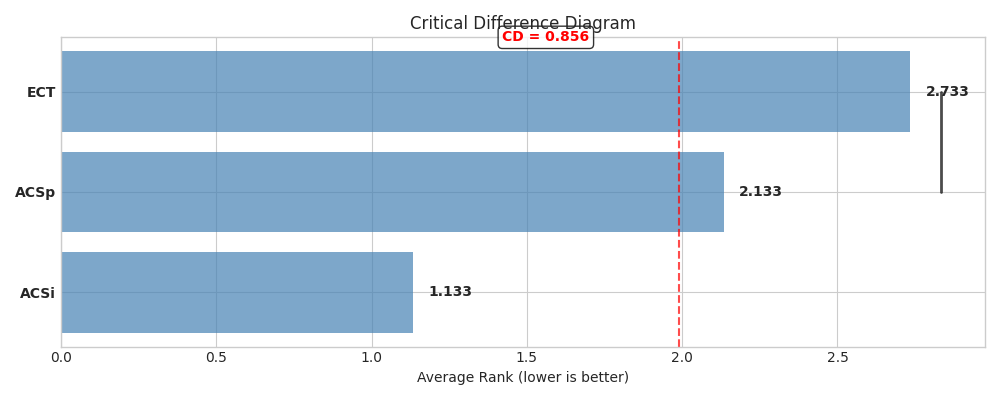
\includegraphics[width=0.9\textwidth]{critical_difference.png}
\caption{Critical Difference diagram showing statistical comparison of algorithms}
\label{fig:cd}
\end{figure}

\begin{figure}[H]
\centering
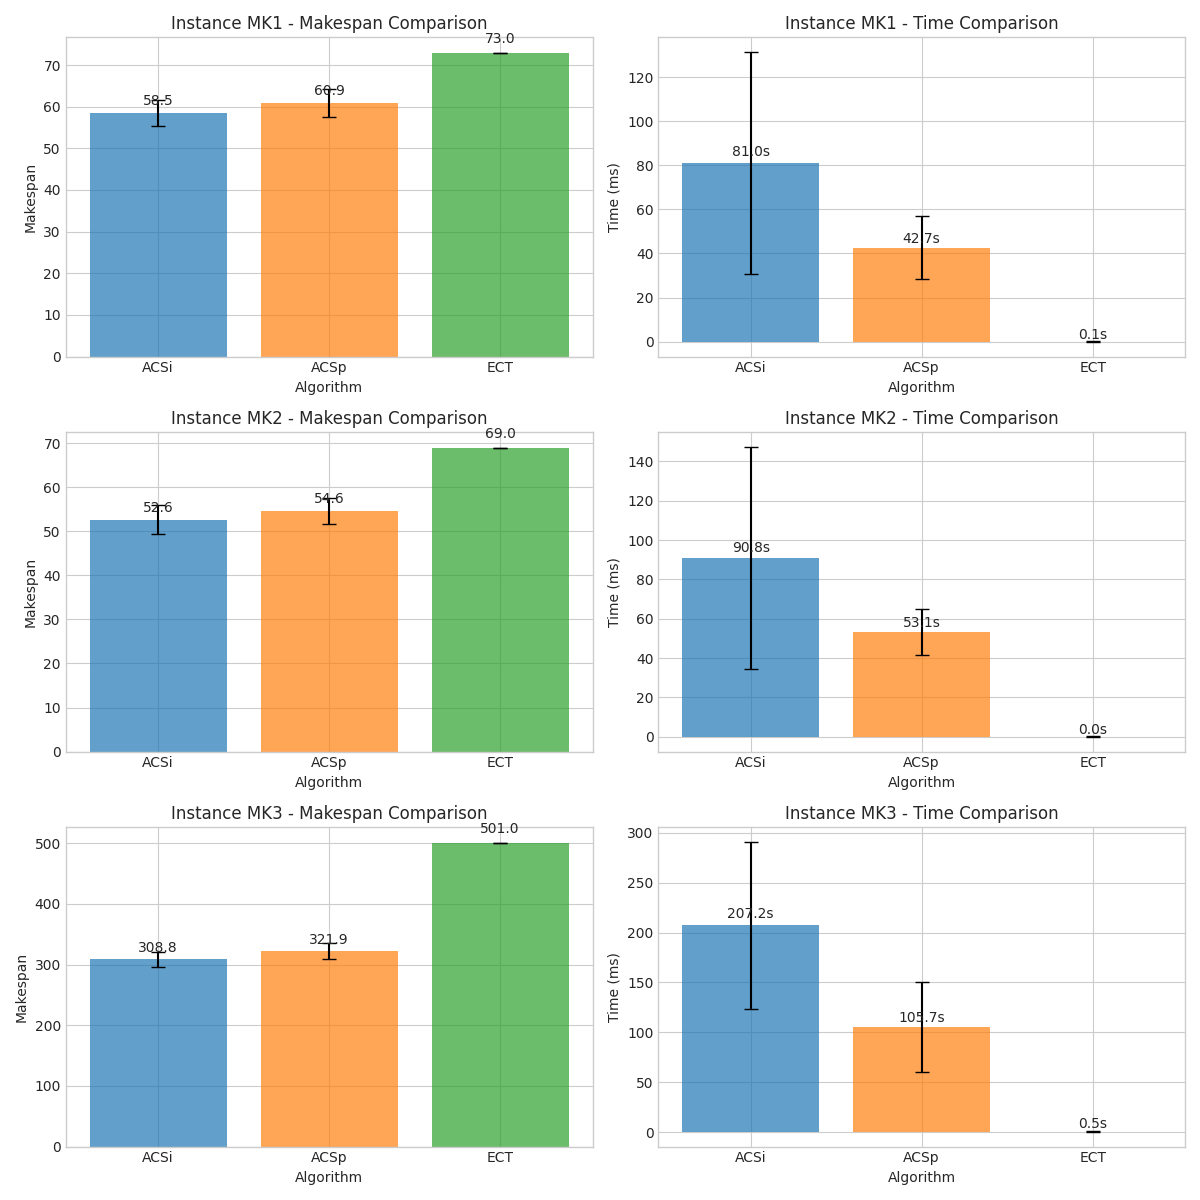
\includegraphics[width=0.9\textwidth]{performance_comparison.png}
\caption{Comparison of makespan and execution time for selected instances}
\label{fig:perf}
\end{figure}

\begin{figure}[H]
\centering
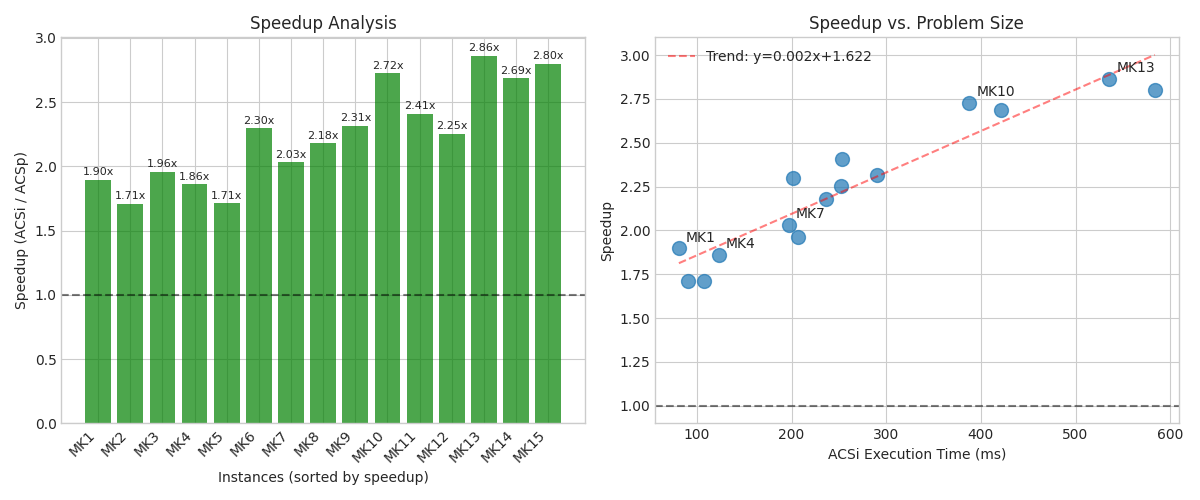
\includegraphics[width=0.9\textwidth]{speedup_analysis.png}
\caption{Speedup analysis of parallel implementation}
\label{fig:speedup}
\end{figure}

\end{document}
